\documentclass[AutoFakeBold,AutoFakeSlant]{beamer}
\usepackage{ctex}
\usepackage{hyperref}
\usepackage[defaultsans]{droidsans}
\usepackage{fontspec}
\usepackage{newtxmath}
\usepackage{latexsym,amsmath,xcolor,multicol,booktabs,calligra,tcolorbox}
\usepackage{graphicx,tabularx,multirow,makecell}
\usepackage{listings}
\usepackage{tikz}
\usetikzlibrary{arrows.meta,positioning}
\lstset{basicstyle=\ttfamily\tiny,breaklines=true,breakatwhitespace=true,columns=fullflexible,frame=single,backgroundcolor=\color{gray!6}}
\usetheme{Madrid}
\usecolortheme{default}
\setbeamertemplate{navigation symbols}{}
\setbeamertemplate{footline}[frame number]
\graphicspath{{./figures_part1/}{../src/analyzer/output/run_20260427_001723/}}

\author{李禹江，张博涵，蒋兴宇}
\title{Part1：隐私政策文本分析与权利识别}
\subtitle{基于 run\_audit.py Prompt 的同意权、访问/查询权、删除权、知情权识别}
\institute{我的刀盾队}
\date{2026-04-27}

\begin{document}
\kaishu

\begin{frame}
    \titlepage
\end{frame}

\begin{frame}
    \frametitle{目录}
    \tableofcontents
\end{frame}

\section{实验定位}

\begin{frame}
    \frametitle{本次实验主题：隐私政策文本分析 + Prompt 工程}
    \small
    \begin{itemize}
        \item \textbf{实验目标}：从隐私政策句子中识别用户权利文本，重点关注同意权、访问/查询权、删除权、知情权。
        \item \textbf{核心问题}：政策是否只是“声明权利”，还是同时给出可执行路径、渠道、数据对象和处理时限。
        \item \textbf{主要方法}：使用 \texttt{run\_audit.py} 中的 LLM prompt；通过法条口径、字段枚举和 few-shot 示例约束输出。
        \item \textbf{产出形式}：每句生成结构化 JSON，并落到 CSV 字段中，支持统计分析、人工复核和后续动态验证。
    \end{itemize}
\end{frame}

\begin{frame}
    \frametitle{实验手册口径与本次实现对应}
    \small
    \begin{tabularx}{\textwidth}{|p{0.24\textwidth}|X|}
        \toprule
        \textbf{汇报要点} & \textbf{本次 Part1 覆盖内容} \\
        \midrule
        实验目的 & 识别隐私政策中同意权、访问/查询权、删除权、知情权等用户权利文本 \\
        \midrule
        实验环境 & Windows + Python；DeepSeek 作为 LLM 后端；BGE 句向量与聚类辅助上下文 \\
        \midrule
        实验内容 & 使用 \texttt{run\_audit.py} prompt 做句级权利识别，支持 few-shot 与同簇上下文 \\
        \midrule
        实验结果 & 23 款应用、9639 句；输出 right\_claim、right\_types、method\_claim、path\_text 等字段 \\
        \midrule
        后续思路 & 用人工标注和动态验证校准 prompt 边界，形成“文本识别—验证—修正”的闭环 \\
        \bottomrule
    \end{tabularx}
\end{frame}

\section{Prompt 设计}

\begin{frame}[fragile]
    \frametitle{Prompt 来源：run\_audit.py 的角色与任务约束}
    \small
    \begin{itemize}
        \item \textbf{System Prompt}：模型被限定为“中文 Android 隐私政策与用户隐私权执行方式分析助手”。
        \item \textbf{法律依据}：以《个人信息保护法》中的个人信息、个人信息处理、用户权利为判断基础。
        \item \textbf{分析对象}：不是整篇政策一次性判断，而是逐句识别用户权利、执行渠道、动态验证目标与可用性风险。
        \item \textbf{工程要求}：只输出严格 JSON，便于后处理为 CSV 字段并做批量统计。
    \end{itemize}
    \vspace{0.3em}
    \begin{lstlisting}
{"right_claim":1,"method_claim":1,"right_types":["access_copy"],"path_text":"账号资料页","usability_risk":"medium"}
    \end{lstlisting}
\end{frame}

\begin{frame}
    \frametitle{识别对象：四类重点权利文本}
    \small
    \begin{tabularx}{\textwidth}{|p{0.22\textwidth}|X|p{0.24\textwidth}|}
        \toprule
        \textbf{权利类型} & \textbf{Prompt 判标口径} & \textbf{典型关键词/路径} \\
        \midrule
        知情权/决定权 & 告知收集哪些数据、为何收集、如何使用、存储、共享、删除；或提供限制/拒绝控制 & 收集、使用、共享、目的、范围、关闭 \\
        \midrule
        同意权/撤回同意 & 用户可同意、拒绝、授权、关闭、撤回授权或调整权限 & 同意、授权、拒绝、撤回、关闭 \\
        \midrule
        访问权/查询权 & 用户可查询、查阅、访问、复制、下载或导出个人信息 & 查询、查阅、访问、复制、下载副本、导出数据 \\
        \midrule
        删除权 & 用户可删除/清除个人信息，或通过注销账号实现删除/匿名化 & 删除、清除、注销账号、匿名化 \\
        \bottomrule
    \end{tabularx}
\end{frame}

\begin{frame}
    \frametitle{结构化字段：把权利识别落到可分析数据}
    \small
    \begin{columns}
        \begin{column}{0.48\textwidth}
            \begin{itemize}
                \item \textbf{right\_claim}：是否出现用户权利、数据控制或知情内容。
                \item \textbf{right\_types}：枚举同意、访问复制、删除、注销等权利类别。
                \item \textbf{method\_claim}：是否给出路径、入口、邮箱、网页、客服或处理时限。
            \end{itemize}
        \end{column}
        \begin{column}{0.48\textwidth}
            \begin{itemize}
                \item \textbf{path\_text}：摘录最具体的执行路径或联系方式。
                \item \textbf{target\_data}：抽取权利指向的数据对象。
                \item \textbf{app\_test\_candidate}：判断是否适合进入 Appium/网页/人工验证。
            \end{itemize}
        \end{column}
    \end{columns}
\end{frame}

\begin{frame}
    \frametitle{Few-shot：用样例固定判标边界}
    \small
    \begin{itemize}
        \item \textbf{作用}：让模型区分“空泛声明权利”和“给出可执行路径”的差异。
        \item \textbf{样例覆盖}：低风险 App 内路径、邮箱/客服渠道、笼统“联系我们”、查询但不可导出、可下载个人信息副本、注销删除等。
        \item \textbf{访问/查询细分}：通过 \texttt{access\_copy\_type} 区分 \texttt{copy}、\texttt{non\_copy}、\texttt{unknown}。
        \item \textbf{后续迭代}：把人工复核中的误判样例补回 few-shot，提升边界一致性。
    \end{itemize}
\end{frame}

\begin{frame}
    \frametitle{端到端流程：Prompt 位于流水线核心}
    \centering
    \begin{tikzpicture}[
        node distance=5mm and 6mm,
        box/.style={draw, rounded corners, align=center, minimum width=2.2cm, minimum height=7.5mm, font=\scriptsize},
        arr/.style={-{Latex[length=1.6mm]}, thick},
    ]
        \node[box, fill=blue!8] (raw) {原始政策};
        \node[box, fill=blue!10, right=of raw] (split) {句子切分};
        \node[box, fill=green!14, right=of split] (cls) {权利文本\\Prompt};
        \node[box, fill=cyan!12, below=of cls] (ctx) {同簇上下文};
        \node[box, fill=orange!16, left=of ctx] (audit) {执行方式\\抽取};
        \node[box, fill=violet!10, left=of audit] (json) {JSON 解析\\统计图表};
        \node[box, fill=yellow!18, below=of audit] (label) {送标队列};
        \node[box, fill=red!12, right=of label] (next) {人工复核\\Few-shot 迭代};
        \draw[arr] (raw) -- (split);
        \draw[arr] (split) -- (cls);
        \draw[arr] (cls) -- (ctx);
        \draw[arr] (ctx) -- (audit);
        \draw[arr] (audit) -- (json);
        \draw[arr] (audit) -- (label);
        \draw[arr] (label) -- (next);
    \end{tikzpicture}
\end{frame}

\section{实验结果}

\begin{frame}
    \frametitle{实验设置与整体规模}
    \small
    \begin{itemize}
        \item \textbf{运行目录}：\texttt{run\_20260427\_001723}。
        \item \textbf{LLM 后端}：DeepSeek；\textbf{审计 prompt}：来自 \texttt{run\_audit.py}；\textbf{limit}：0，即全量运行。
        \item \textbf{Few-shot}：在 prompt 中内置多类权利执行样例；分类阶段也支持外部 shots 注入。
        \item \textbf{上下文}：审计前聚类开启，把同簇句子作为参考上下文，最终仍只给当前句打标。
        \item \textbf{数据规模}：23 款应用，共 9639 句；累计送标候选 4371 条。
    \end{itemize}
    \centering
    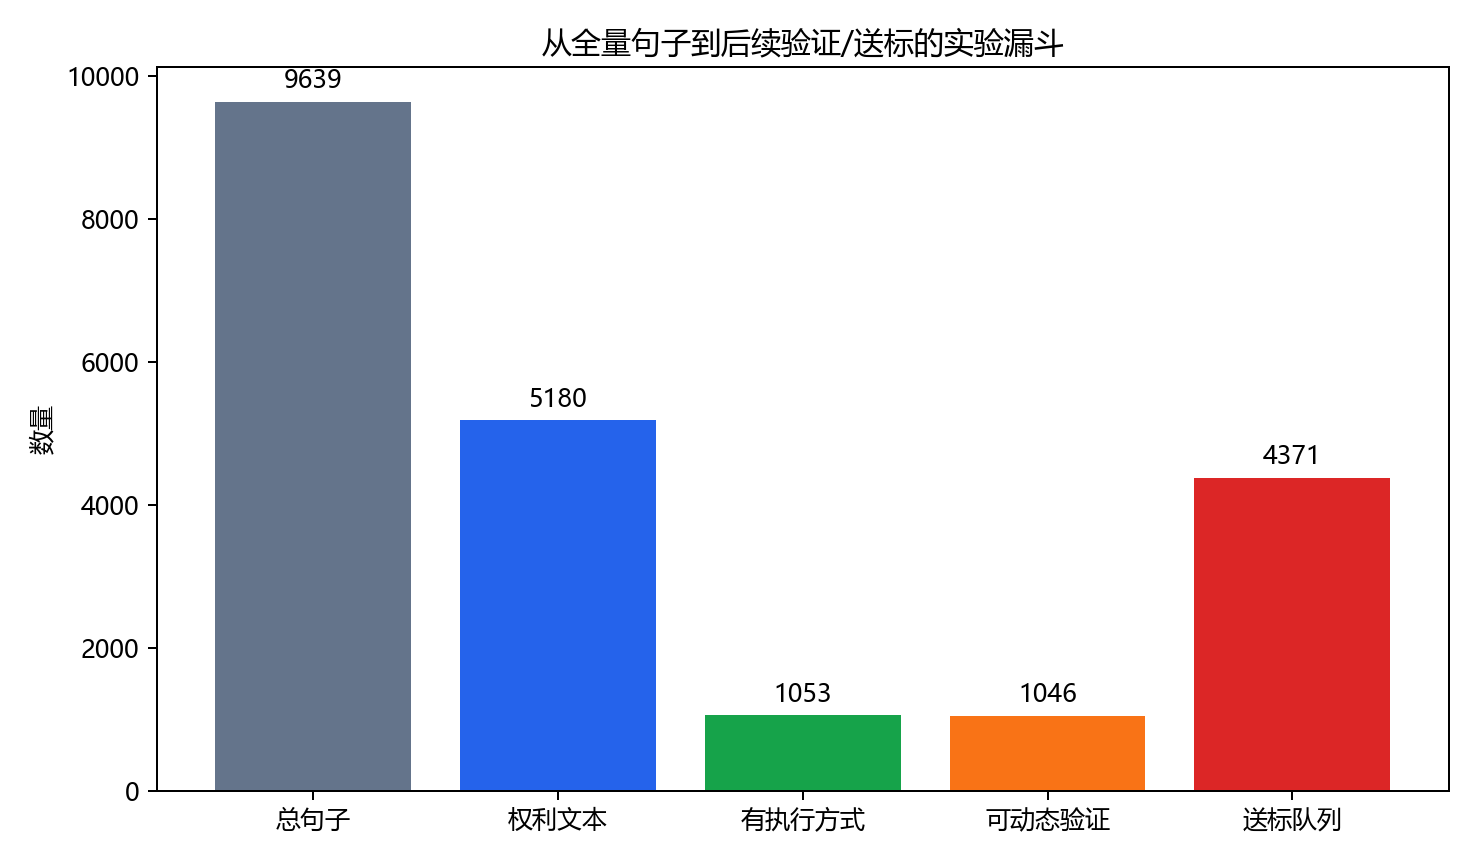
\includegraphics[width=0.82\linewidth]{fig_part1_funnel.png}
\end{frame}

\begin{frame}
    \frametitle{数据规模：句子数 Top 10}
    \centering
    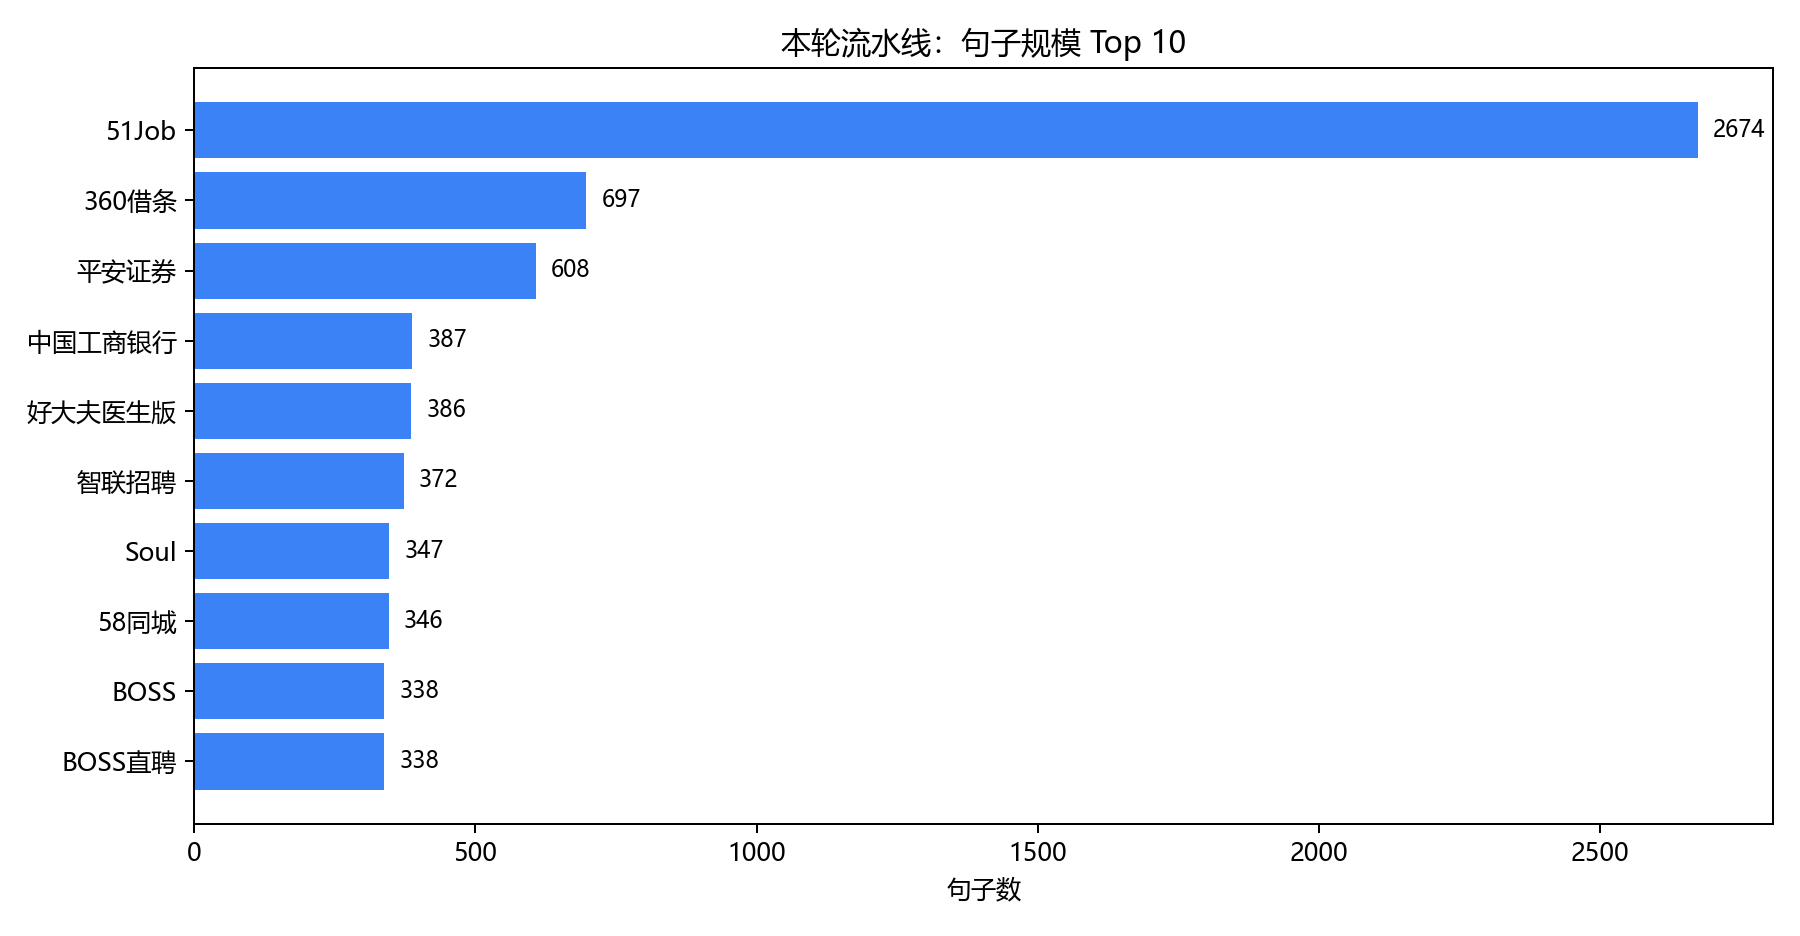
\includegraphics[width=0.92\linewidth]{fig_part1_sentence_top10.png}
\end{frame}

\begin{frame}
    \frametitle{Prompt 输出结果：主要标签正例率}
    \centering
    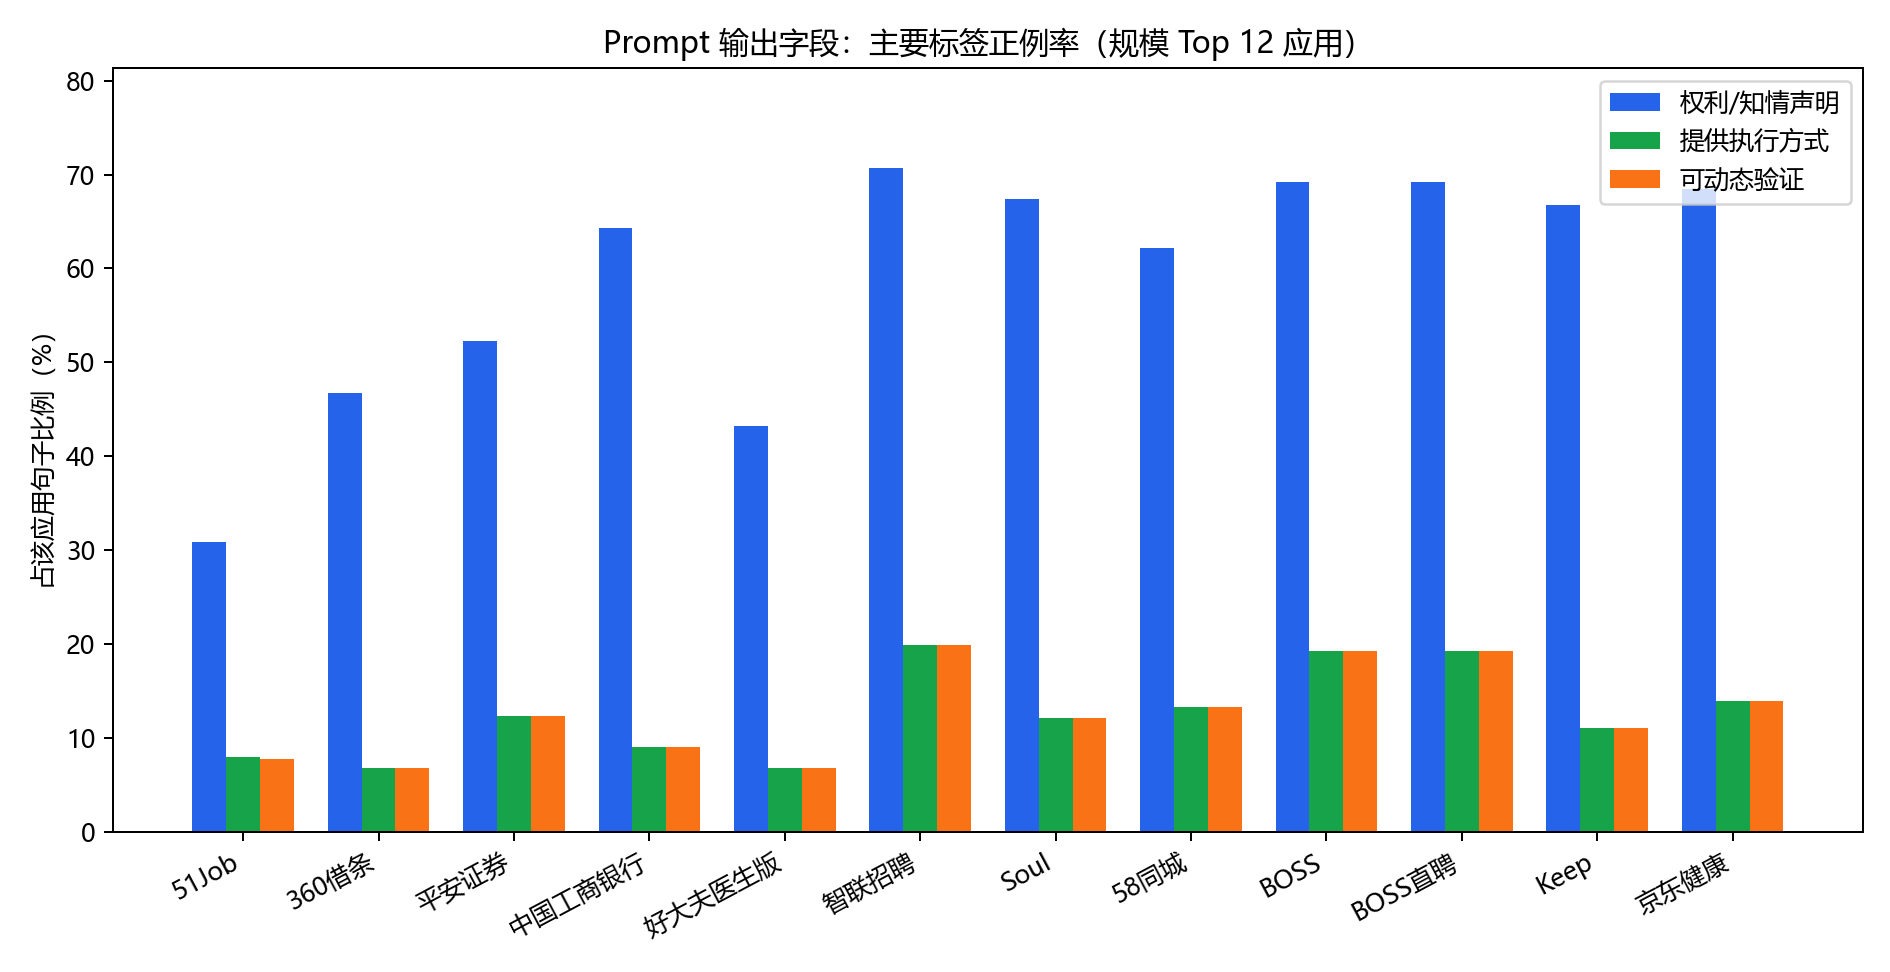
\includegraphics[width=0.96\linewidth]{fig_part1_claim_rates_top12.png}
    \vspace{0.2em}
    \scriptsize
    结果显示，\textbf{right\_claim} 主要捕捉权利/知情文本，\textbf{method\_claim} 和 \textbf{app\_test\_candidate} 更关注是否给出可执行路径。
\end{frame}

\begin{frame}
    \frametitle{重点权利类型识别结果}
    \centering
    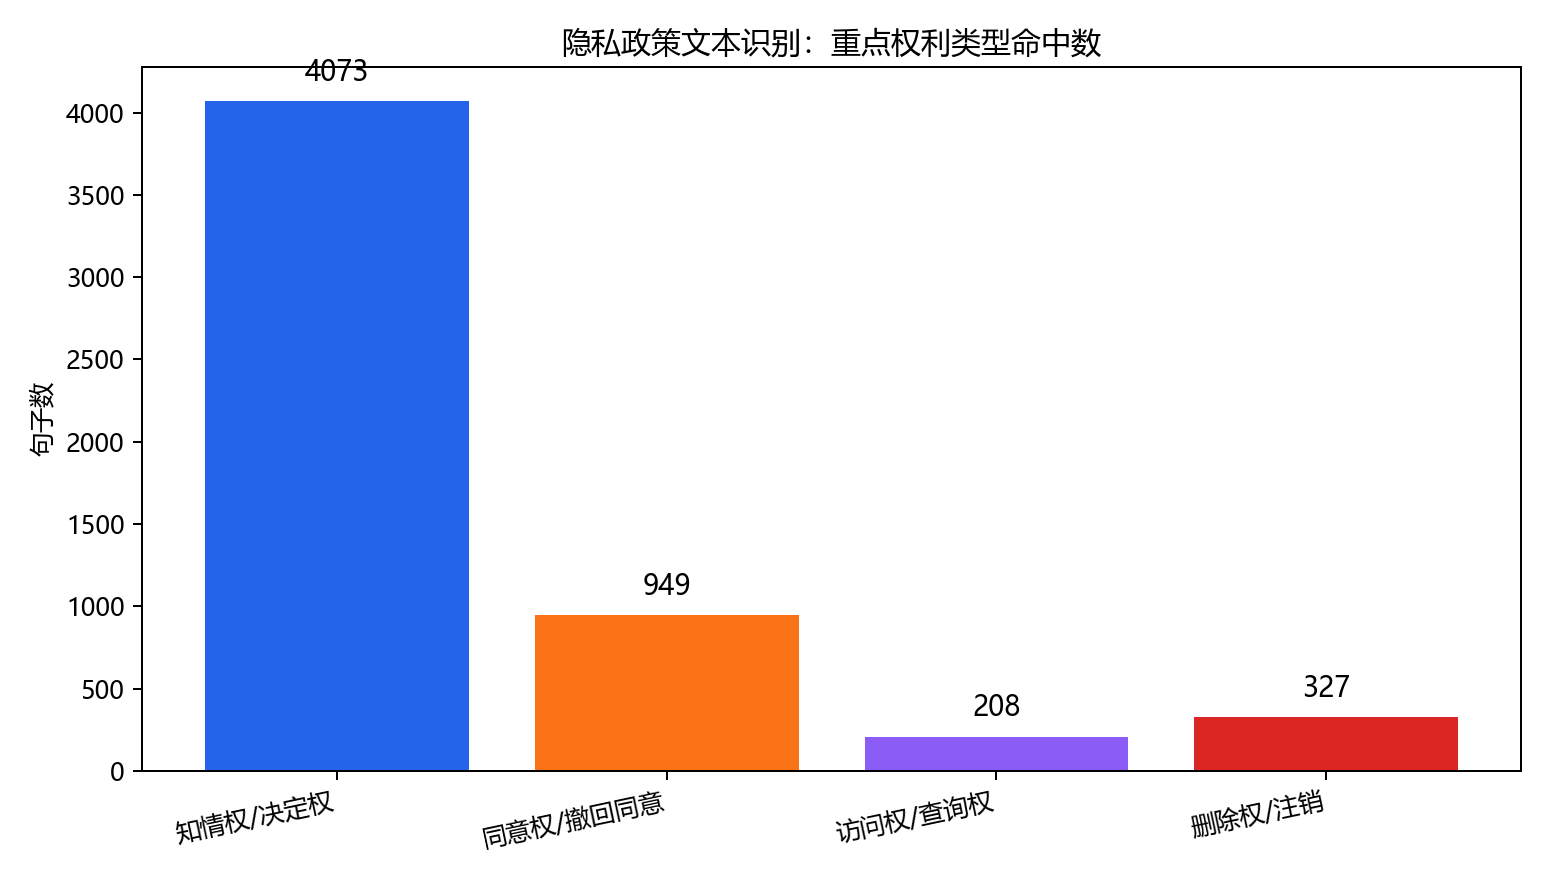
\includegraphics[width=0.9\linewidth]{fig_part1_right_focus_counts.png}
    \vspace{0.2em}
    \scriptsize
    同一句可能同时命中多个 \texttt{right\_types}，因此各类权利计数之和可能大于 \texttt{right\_claim} 总数。
\end{frame}

\begin{frame}
    \frametitle{Top 应用统计表}
    \tiny
    \begin{tabularx}{\textwidth}{|l|r|r|r|r|r|}
        \toprule
        \textbf{应用} & \textbf{句数} & \textbf{right} & \textbf{method} & \textbf{candidate} & \textbf{method率} \\
        \midrule
        51Job & 2674 & 826 & 213 & 207 & 8.0\% \\
        360借条 & 697 & 326 & 47 & 47 & 6.7\% \\
        平安证券 & 608 & 318 & 75 & 75 & 12.3\% \\
        中国工商银行 & 387 & 249 & 35 & 35 & 9.0\% \\
        好大夫医生版 & 386 & 167 & 26 & 26 & 6.7\% \\
        智联招聘 & 372 & 263 & 74 & 74 & 19.9\% \\
        Soul & 347 & 234 & 42 & 42 & 12.1\% \\
        58同城 & 346 & 215 & 46 & 46 & 13.3\% \\
        \midrule
        \textbf{合计} & \textbf{9639} & \textbf{5180} & \textbf{1053} & \textbf{1046} & \textbf{10.9\%} \\
        \bottomrule
    \end{tabularx}
    \vspace{0.35em}
    \scriptsize
    观察：权利文本数量较高，但真正给出执行路径的句子占比明显更低，这说明 Prompt 需要把“有权利声明”和“可操作路径”分开抽取。
\end{frame}

\begin{frame}
    \frametitle{访问复制权：副本形态进一步细分}
    \begin{columns}
        \begin{column}{0.52\textwidth}
            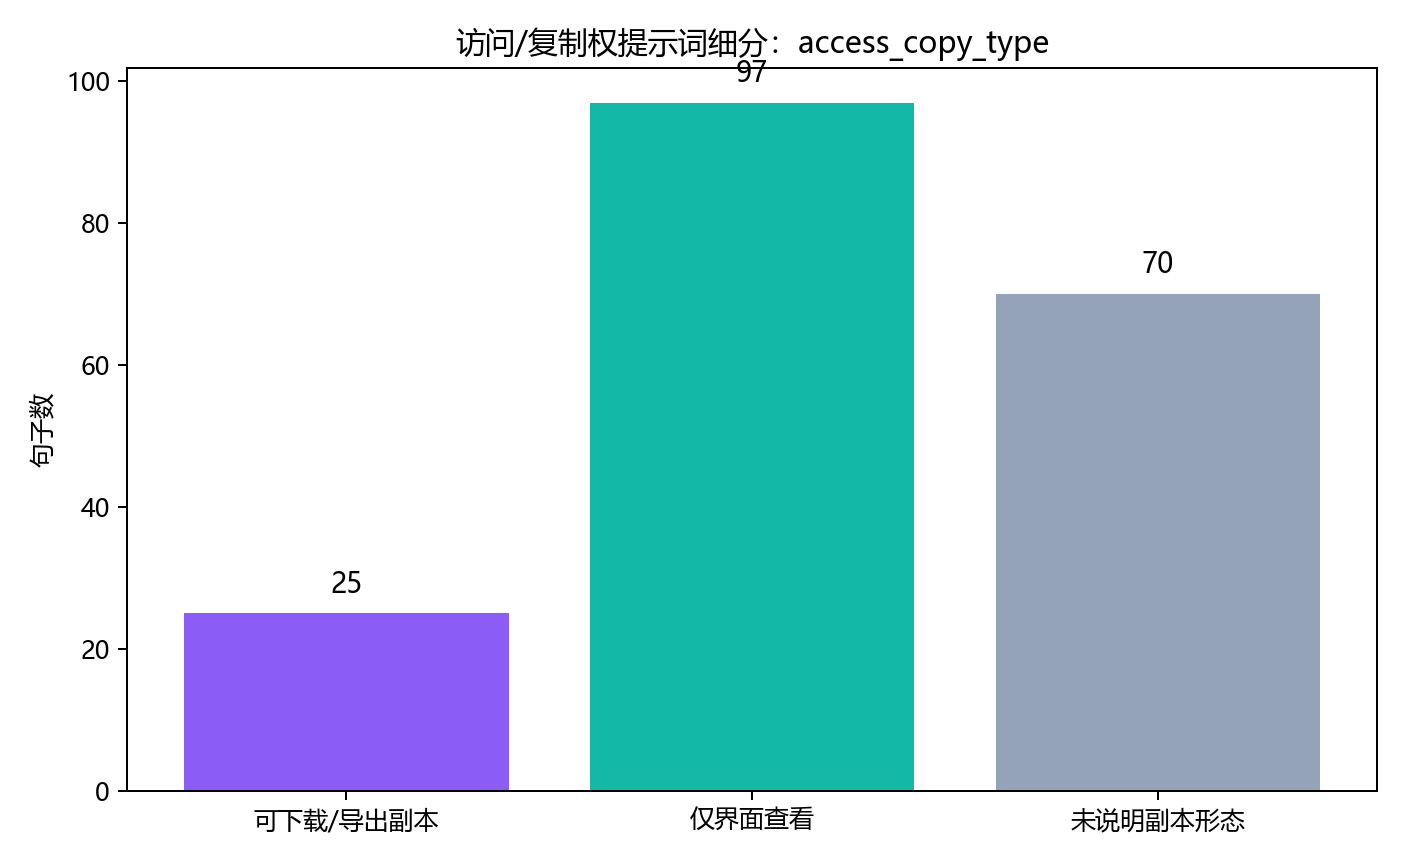
\includegraphics[width=\linewidth]{fig_part1_access_copy_type.png}
        \end{column}
        \begin{column}{0.45\textwidth}
            \small
            \begin{itemize}
                \item \textbf{copy}：能下载、导出、保存为副本，适合验证数据可携带性。
                \item \textbf{non\_copy}：只能在界面内查看，常见于账号资料页。
                \item \textbf{unknown}：只声明查阅/复制权，但未说明路径或副本形态。
            \end{itemize}
        \end{column}
    \end{columns}
\end{frame}

\begin{frame}
    \frametitle{执行方式识别率较高的应用}
    \tiny
    \begin{tabularx}{\textwidth}{|l|r|r|r|r|}
        \toprule
        \textbf{应用} & \textbf{句数} & \textbf{method} & \textbf{method率} & \textbf{copy/non/unknown} \\
        \midrule
        智联招聘 & 372 & 74 & 19.9\% & 4/4/6 \\
        BOSS & 338 & 65 & 19.2\% & 0/8/4 \\
        BOSS直聘 & 338 & 65 & 19.2\% & 0/8/4 \\
        心脏健康研究 & 73 & 12 & 16.4\% & 0/1/2 \\
        支付宝 & 247 & 35 & 14.2\% & 1/1/0 \\
        Blued极速版 & 192 & 27 & 14.1\% & 0/2/2 \\
        \bottomrule
    \end{tabularx}
    \vspace{0.4em}
    \scriptsize
    这类应用适合作为后续动态验证的优先样本，因为 Prompt 已抽取出较多路径、渠道或测试目标。
\end{frame}

\section{总结与后续}

\begin{frame}
    \frametitle{阶段性结论}
    \small
    \begin{itemize}
        \item \textbf{实验对象更明确}：本轮不是泛化的隐私分类，而是面向同意、访问/查询、删除、知情等用户权利文本识别。
        \item \textbf{Prompt 输出可解释}：\texttt{right\_types} 说明“识别到什么权利”，\texttt{path\_text} 说明“用户如何执行”。
        \item \textbf{结果可进入下一阶段}：\texttt{dynamic\_test\_goal} 与 \texttt{app\_test\_candidate} 可转化为 Appium/网页/人工核查清单。
        \item \textbf{Few-shot 是主要迭代入口}：人工复核后的分歧样例可以持续补强 prompt 的边界案例。
    \end{itemize}
\end{frame}

\begin{frame}
    \frametitle{实验过程和结构还可提高的地方}
    \small
    \begin{itemize}
        \item \textbf{建立人工真值集}：每类权利抽样标注，分别评估同意权、访问/查询权、删除权、知情权的 Precision/Recall/F1。
        \item \textbf{拆分 prompt 任务}：先识别权利类型，再抽取路径/渠道/数据对象，降低一个 prompt 同时完成多任务的混淆。
        \item \textbf{Few-shot 分层}：按权利类型维护示例库，尤其补足“只有权利声明但无路径”“查询但不可导出”“删除依赖客服”等边界例。
        \item \textbf{增加一致性检查}：同一句多次推理或多模型交叉验证，对不稳定样本优先送标。
        \item \textbf{闭环验证}：将 \texttt{app\_test\_candidate=1} 转为动态测试任务，记录政策路径在真实 App/网页中是否存在、是否可达。
    \end{itemize}
\end{frame}

\begin{frame}
    \frametitle{后续实验路线}
    \small
    \begin{enumerate}
        \item 从本轮结果中按权利类型与风险等级抽样，形成小规模人工金标集。
        \item 基于误检/漏检样例重写 few-shot，分权利类型迭代 prompt。
        \item 对有明确路径的样本做 Appium/网页验证，检查“文本承诺”与“实际入口”是否一致。
        \item 将文本识别、人工标注、动态验证结果合并，形成最终可解释的隐私权利执行评估报告。
    \end{enumerate}
\end{frame}

\begin{frame}
    \begin{center}
        {\Huge 感谢聆听！}
    \end{center}
\end{frame}

\end{document}
